%!TEX program = xelatex
\documentclass[times,namecite]{goose-article}

\title{%
  GMatElastoPlasticQPot3d -- An implementation for an elasto-plastic continuum model based on a manifold of quadratic potentials
}

\author{T.W.J.~de~Geus}

\contact{%
  $^*$Contact: %
  \href{mailto:tom@geus.me}{tom@geus.me} %
  \hspace{1mm}--\hspace{1mm} %
  \href{http://www.geus.me}{www.geus.me}%
  \hspace{1mm}--\hspace{1mm} %
  \href{https://github.com/tdegeus/GMatElastoPlasticQPot3d}{https://github.com/tdegeus/GMatElastoPlasticQPot3d}%
}

\hypersetup{pdfauthor={T.W.J. de Geus}}

\header{%
  \href{https://github.com/tdegeus/GMatElastoPlasticQPot3d}{GMatElastoPlasticQPot3d} -- \href{http://www.geus.me}{T.W.J.\ de Geus}%
}

\newcommand\leftstar[1]{\hspace*{-.3em}~^\star\!#1}

\newcommand\T[1]{\underline{\bm{{#1}}}}

\newcommand\TT[1]{\underline{\mathbb{{#1}}}}

\begin{document}

\maketitle

\begin{abstract}
A microscopic continuum model of plasticity in amorphous solids is proposed. This model uses a strain energy with multiple minima to capture the effect of plasticity. This model is inspired on the work of \citet{Jagla2017}. It is formulated in 3-d, and can consequently be used for 2-d plain strain.
\end{abstract}

\keywords{elasto-plasticity; linear elasticity}

\setcounter{tocdepth}{3}
\tableofcontents

\vfill\newpage
\section{Introduction}

The model is constructed such that it behaves linear elastically in the volumetric stress response. The same holds for the deviatoric stress response, whereby plasticity is modelled such that the material starts flowing once a critical strain is reached. After a period of flow, the deviatoric stress response is again linear elastic.

\section{Linear elasticity}

The model is an extension of linear elasticity, which is defined in terms of the following strain energy density
\begin{equation}
\label{eq:energy:elastic}
  W = \tfrac{1}{2} \lambda \left( \mathrm{tr} ( \T{\varepsilon} ) \right)^2 + \mu \, \T{\varepsilon} : \T{\varepsilon}
\end{equation}
where $\lambda$ and $\mu$ are Lam\'{e}'s constants (see appendices for the rest of the nomenclature). This corresponds to the following stress tensor
\begin{equation}
  \T{\sigma} \equiv \frac{\partial W}{\partial \T{\varepsilon}}
  = \lambda \, \mathrm{tr} ( \T{\varepsilon} ) \T{I} + 2 \mu \, \T{\varepsilon}
\end{equation}
This can be reorganised (using $\lambda \equiv \kappa - 2/3 \mu$) to be an additive decomposition of a purely volumetric stress and a purely deviatoric stress:
\begin{align}
  \T{\sigma}
  &= \left( \kappa - \tfrac{2}{3} \mu \right) \, \mathrm{tr} ( \T{\varepsilon} ) \T{I} + 2 \mu \, \T{\varepsilon}
  \\
  &= \kappa \, \mathrm{tr} ( \T{\varepsilon} ) \T{I} + 2 \mu \left( \T{\varepsilon} - \tfrac{1}{3} \mathrm{tr} ( \T{\varepsilon} ) \T{I} \right)
  \\
  &= \kappa \, \mathrm{tr} ( \T{\varepsilon} ) \T{I} + 2 \mu \, \T{\varepsilon}_\mathrm{d}
\end{align}
Here, $\kappa$ is the bulk modulus: the ratio of pressure and volumetric strain; $\mu$ is the shear modulus: the ratio of shear stress and shear strains, contained in the strain deviator
\begin{equation}
  \T{\varepsilon}_\mathrm{d} \equiv \T{\varepsilon} - \tfrac{1}{3} \mathrm{tr} ( \T{\varepsilon} ) \T{I}
\end{equation}

\section{Equivalent deviatoric (shear) strain}

Eq.~\eqref{eq:energy:elastic} is actually a quadratic potential in both volumetric and shear strain space. To emphasise the latter it is useful to introduce an equivalent deviatoric strain
\begin{equation}
  \varepsilon_\mathrm{d} \equiv \sqrt{ \tfrac{1}{2} \T{\varepsilon}_\mathrm{d} : \T{\varepsilon}_\mathrm{d} }
\end{equation}
It contains the amplitude of the deviatoric (shear) strains, i.e.\
\begin{equation}
  \T{\varepsilon}_\mathrm{d} = \varepsilon_\mathrm{d} \T{N}_\mathrm{d}
\end{equation}
where the direction of shear is contained in
\begin{equation}
  \T{N}_\mathrm{d} \equiv \frac{\T{\varepsilon}_\mathrm{d}}{\varepsilon_\mathrm{d}}
\end{equation}
Note that
\begin{equation}
  \sqrt{ \tfrac{1}{2} \T{N}_\mathrm{d} : \T{N}_\mathrm{d} } = 1,
  \qquad
  \frac{\partial \varepsilon_\mathrm{d}}{\partial \T{\varepsilon}_\mathrm{d}} = \tfrac{1}{2} \T{N}_\mathrm{d}
\end{equation}
(see Appendix~\ref{sec:nomenclature:derivatives}). Using this definition the elastic strain energy can be rewritten as
\begin{equation}
  W = \tfrac{1}{2} \kappa \left( \mathrm{tr} ( \T{\varepsilon} ) \right)^2 + 2 \mu \varepsilon_\mathrm{d}^2
\end{equation}
One now easily recognises a sum of two quadratic potentials:
\begin{equation}
  W = U ( \varepsilon_\mathrm{m} ) + V ( \varepsilon_\mathrm{d} )
\end{equation}
with
\begin{equation}
\label{eq:potentials:elastic}
  U ( \varepsilon_\mathrm{m} ) = \tfrac{9}{2} \kappa \, \varepsilon_\mathrm{m}^2,
  \qquad
  V ( \varepsilon_\mathrm{d} ) = 2 \mu \, \varepsilon_\mathrm{d}^2
\end{equation}
where $\varepsilon_\mathrm{m} \equiv \mathrm{tr} ( \T{\varepsilon} ) / 3$. Both quadratic potentials have been plotted in Fig.~\ref{fig:U-V:elas}, and their derivatives in equivalent strain space in Fig.~\ref{fig:dU-dV:elas}.

\begin{figure}[htp]
  \centering
  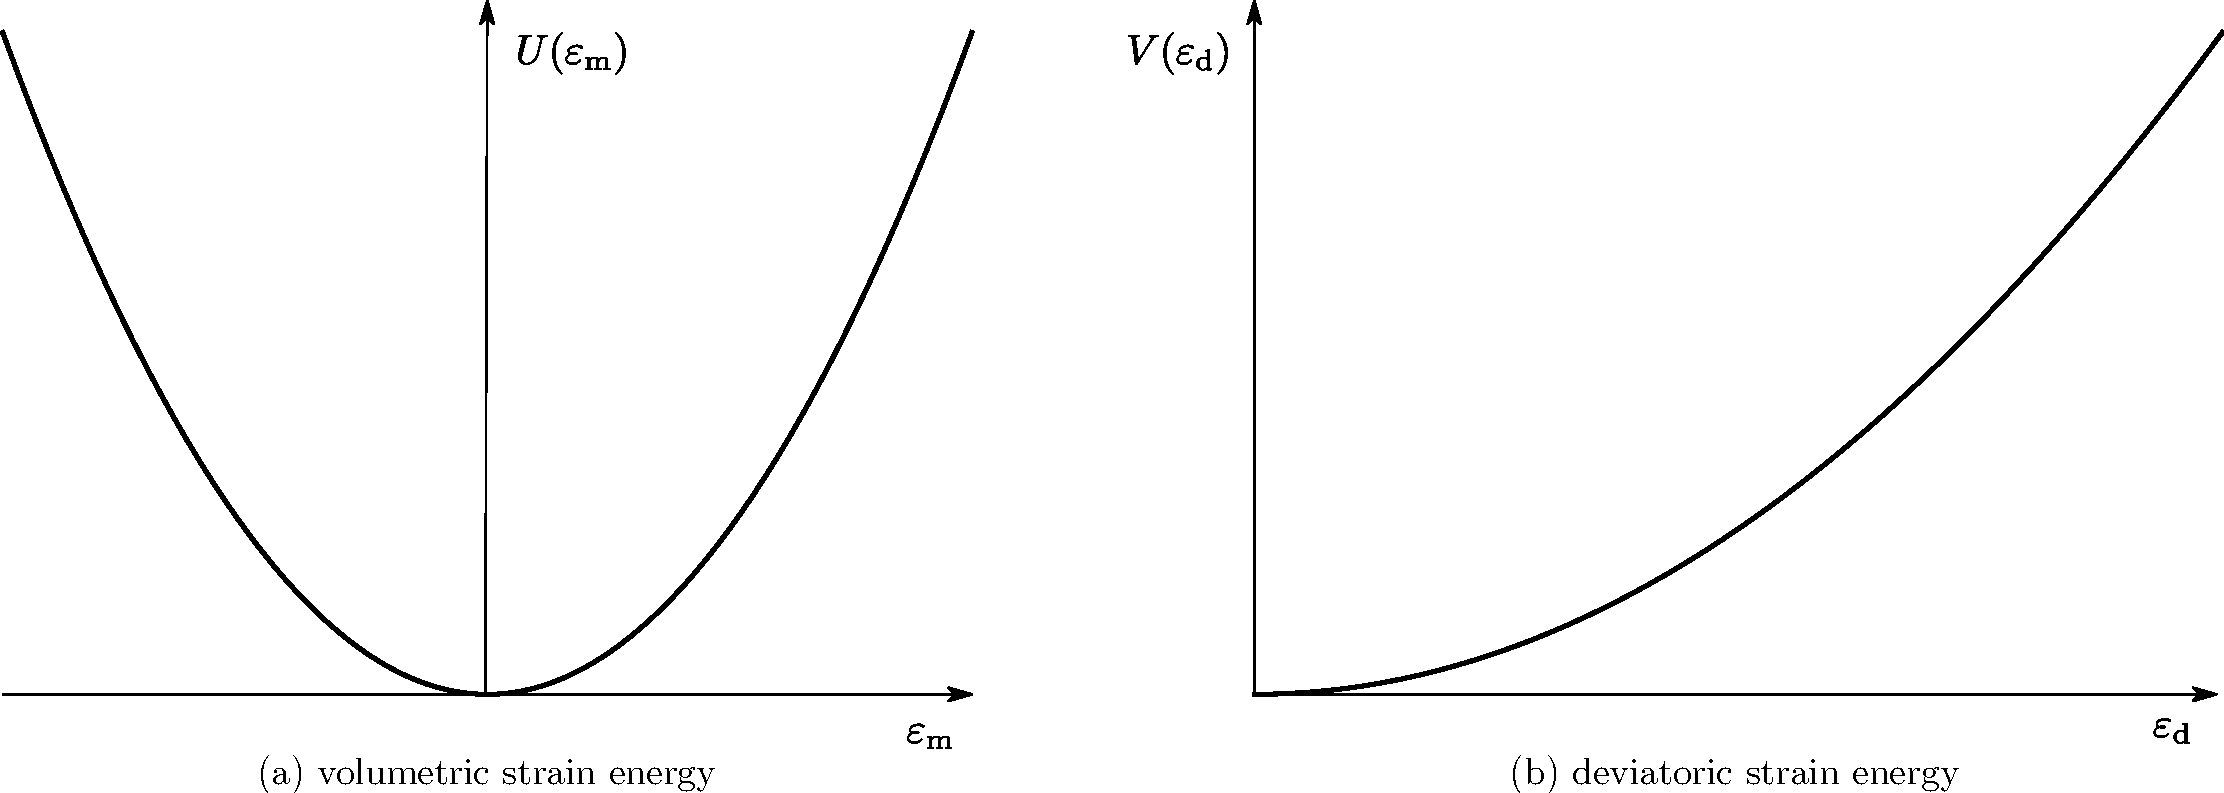
\includegraphics[width=1.\textwidth]{figures/potential_U-V_elas}
  \caption{Strain energy $W ( \T{\varepsilon} ) = U ( \varepsilon_\mathrm{m} ) + V ( \varepsilon_\mathrm{d} )$ for linear elasticity.}
  \label{fig:U-V:elas}
\end{figure}

\begin{figure}[htp]
  \centering
  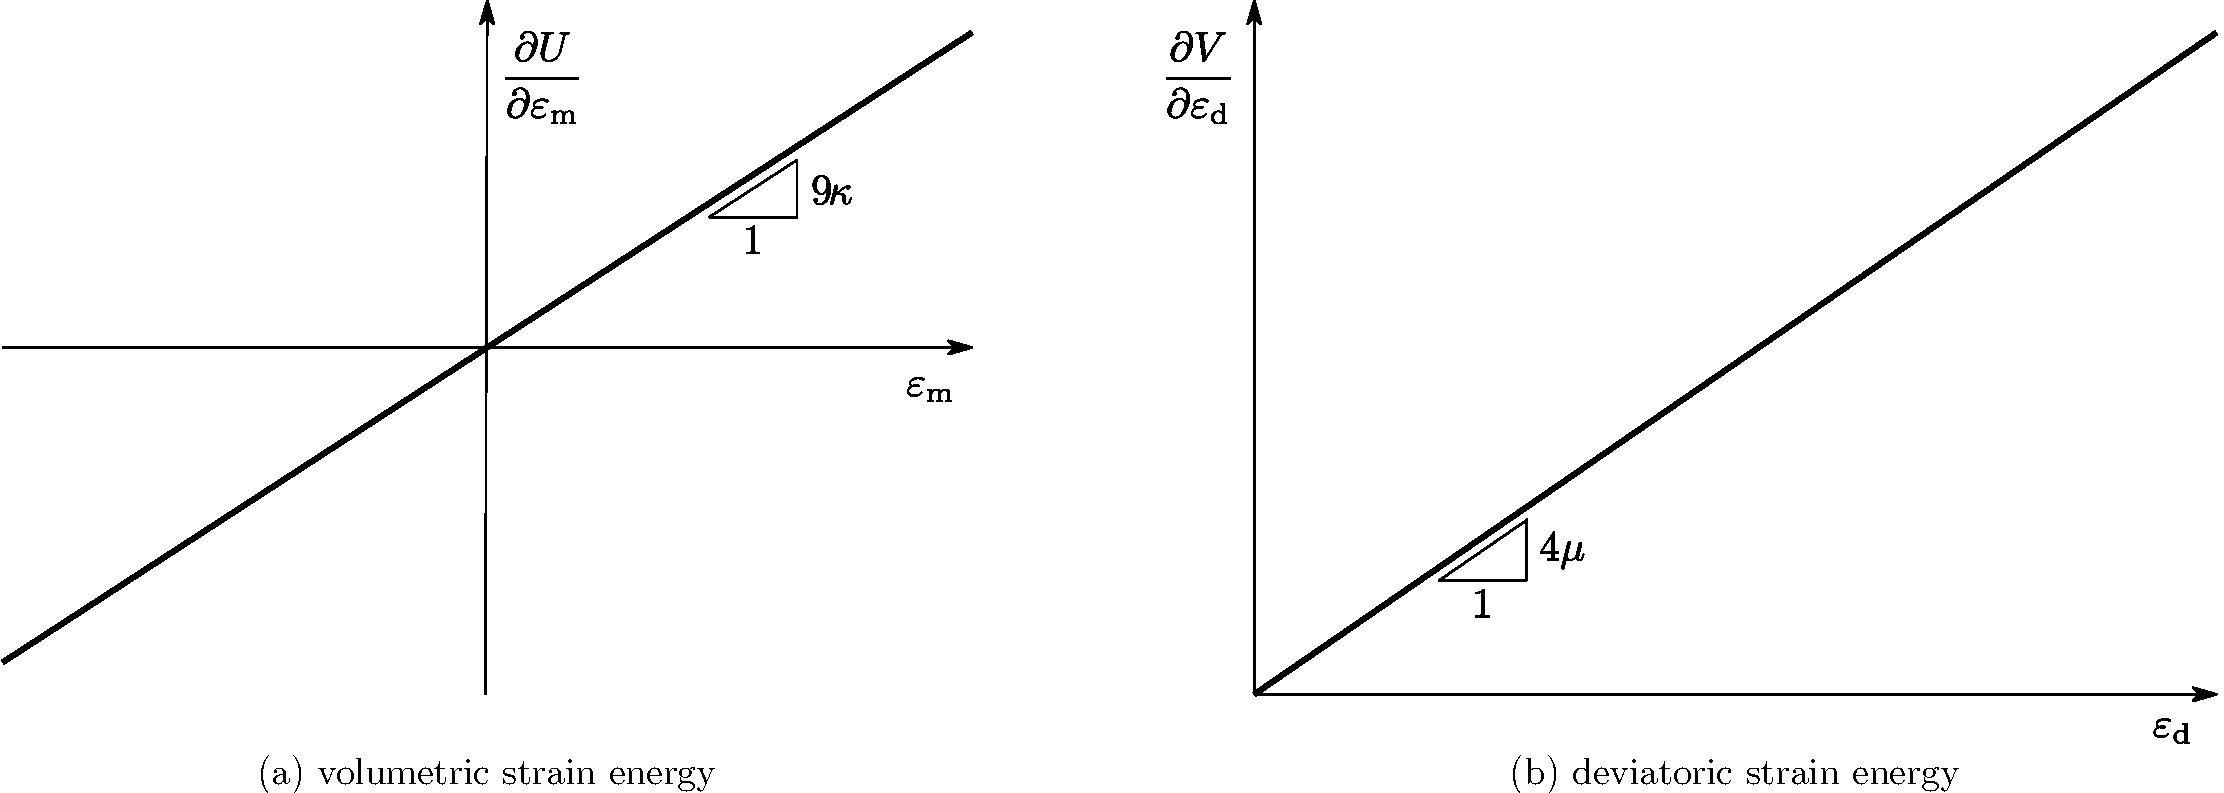
\includegraphics[width=1.\textwidth]{figures/potential_dU-dV_elas}
  \caption{Derivative of the hydrostatic strain energy $U$ and the deviatoric strain energy $V$ w.r.t.\ respectively the hydrostatic strain $\varepsilon_\mathrm{m}$ and the equivalent deviatoric strain $\varepsilon_\mathrm{d}$.}
  \label{fig:dU-dV:elas}
\end{figure}

\section{Plasticity}

The model is now extended to account for plasticity. The model is defined such that the material responds volumetrically purely elastic, while in shear the model is governed by multiple minima. These minima have the effect that when the material reaches a certain yield stress, it jumps to the next minimum. Around this minimum the elasticity is always the same. When loading is continued the material again jumps to a new minimum when the next yield stress is reached. The magnitude of the jumps and of the yield stress are thereby related.

As described, the volumetric behaviour is simply elastic; whereby the potential is given by Eq.~(\ref{eq:potentials:elastic}a) and is plotted in Fig.~\ref{fig:U-V:elas}(a). To attain the desired behaviour in shear, the equivalent deviatoric strain space is divided in a finite number of yield strains $\varepsilon_\mathrm{y}^{(0)}, \varepsilon_\mathrm{y}^{(1)}, \varepsilon_\mathrm{y}^{(2)}, ...$. A parabolic potential is then defined between each pair ($[ \varepsilon_\mathrm{y}^{(0)}, \varepsilon_\mathrm{y}^{(1)} )$, $[ \varepsilon_\mathrm{y}^{(1)}, \varepsilon_\mathrm{y}^{(2)} )$, ...).

The shear strain energy is then composed of a manifold of quadratic contributions
\begin{equation}\label{eq:V-plas}
  V \big(
    \varepsilon_\mathrm{y}^{(i)} \leq \varepsilon_\mathrm{d} < \varepsilon_\mathrm{y}^{(i+1)}
  \big)
  =
  V^{(i)}
  =
  2 \mu \, \bigg[\,
    \Big[\, \varepsilon_\mathrm{d} - \varepsilon_\mathrm{min}^{(i)} \,\Big]^2
    -
    \Big[\, \Delta \varepsilon_\mathrm{y}^{(i)} \,\Big]^2
  \,\bigg]
\end{equation}
where the mean of $\varepsilon_\mathrm{y}^{(i)}$ and $\varepsilon_\mathrm{y}^{(i+1)}$ is
\begin{equation}
  \varepsilon_\mathrm{min}^{(i)}
  =
  \tfrac{1}{2} \Big[\, \varepsilon_\mathrm{y}^{(i+1)} + \varepsilon_\mathrm{y}^{(i)} \,\Big]
\end{equation}
which is also the equivalent deviatoric strain at which the shear strain energy reaches its minimum. It may be interpreted as a plastic strain. From this minimum, the distance to $\varepsilon_\mathrm{y}^{(i)}$ and $\varepsilon_\mathrm{y}^{(i+1)}$ is
\begin{equation}
  \Delta \varepsilon_\mathrm{y}^{(i)}
  =
  \tfrac{1}{2} \Big[\, \varepsilon_\mathrm{y}^{(i+1)} - \varepsilon_\mathrm{y}^{(i)} \,\Big]
\end{equation}
The resulting shear strain energy is plotted in Fig.~\ref{fig:V:plas}(a).

The stress response is obtained using
\begin{equation}\label{eq:dV-plas}
  \frac{\partial V^{(i)}}{\partial \varepsilon_\mathrm{d}}
  =
  4 \mu \, \Big[\, \varepsilon_\mathrm{d} - \varepsilon_\mathrm{min}^{(i)} \,\Big]
\end{equation}
(see Fig.~\ref{fig:dV:plas}(a)). From which it can be observed that in elasticity the behaviour is identical to above (cf.~(\ref{eq:potentials:elastic}b)). For the case that $\varepsilon_\mathrm{y}^{(0)} = - \varepsilon_\mathrm{y}^{(1)}$ the responses are even identical until initial yield stress is reached. The stress finally reads
\begin{equation}
  \T{\sigma} ( \T{\varepsilon} )
  =
  \kappa \, \mathrm{tr} ( \T{\varepsilon} ) \, \T{I}
  +
  2 \mu \, \Big[\, \varepsilon_\mathrm{d} - \varepsilon_\mathrm{min}^{(i)} \,\Big] \;
  \T{N}_\mathrm{d}
  \qquad
  \mathrm{for}
  \;
  \varepsilon_\mathrm{y}^{(i)} \leq \varepsilon_\mathrm{d} < \varepsilon_\mathrm{y}^{(i+1)}
\end{equation}
whereby one has to assume that when $\varepsilon_\mathrm{d} = 0$ also $\T{\sigma}_\mathrm{d} = \T{0}$ in order to avoid zero division. The response is plotted in Fig.~\ref{fig:dV:plas}(a), from which it is observed that it exhibits stress jumps between different parabola in the potential, because of the discontinuity in the second derivative of the elastic potential. This can be remedied, such as in the model presented below.

\section{Plasticity -- smooth potential}

The remedy the discontinuity in the second derivative of the potential, it is smoothed as follows:
\begin{equation}\label{eq:V-plas-smooth}
  V \big(
    \varepsilon_\mathrm{y}^{(i)} \leq \varepsilon_\mathrm{d} < \varepsilon_\mathrm{y}^{(i+1)}
  \big)
  =
  V^{(i)}
  =
  - 4 \mu \,
  \left[ \frac{\Delta \varepsilon_\mathrm{y}^{(i)}}{\pi} \right]^2
  \left[
    1
    +
    \cos \left(
      \frac{ \pi }{ \Delta \varepsilon_\mathrm{y}^{(i)} }
      \Big[\, \varepsilon_\mathrm{d} - \varepsilon_\mathrm{min}^{(i)} \,\Big]
    \right)
  \right]
\end{equation}
which is plotted in Fig.~\ref{fig:V:plas}(b). In this case the stress is obtained from
\begin{equation}\label{eq:dV-plas-smooth}
  \frac{\partial V^{(i)}}{\partial \varepsilon_\mathrm{d}}
  =
  4 \mu \,
  \left[ \frac{\Delta \varepsilon_\mathrm{y}^{(i)}}{\pi} \right]
  \sin \left(
    \frac{ \pi }{ \Delta \varepsilon_\mathrm{y}^{(i)} }
    \Big[\, \varepsilon_\mathrm{d} - \varepsilon_\mathrm{min}^{(i)} \,\Big]
  \right)
\end{equation}
(see Fig.~\ref{fig:dV:plas}(b)). Which is to the first order equal to linear elasticity around its minimum $\varepsilon_\mathrm{min}^{(i)}$. Indeed, the first order Taylor series of Eq.~\eqref{eq:dV-plas-smooth} around $\varepsilon_\mathrm{d} = \varepsilon_\mathrm{min}^{(i)}$,
\begin{equation}
  \frac{\partial V^{(i)}}{\partial \varepsilon_\mathrm{d}}
  \approx
  4 \mu \, \Big[\, \varepsilon_\mathrm{d} - \varepsilon_\mathrm{min}^{(i)} \,\Big]
\end{equation}
is identical to Eq.~\eqref{eq:dV-plas}.

The stress tensor finally reads
\begin{equation}
  \T{\sigma} ( \T{\varepsilon} )
  =
  \kappa \, \mathrm{tr} ( \T{\varepsilon} ) \, \T{I}
  +
  2 \mu \,
  \left[ \frac{\Delta \varepsilon_\mathrm{y}^{(i)}}{\pi} \right]
  \sin \left(
    \frac{ \pi }{ \Delta \varepsilon_\mathrm{y}^{(i)} }
    \Big[\, \varepsilon_\mathrm{d} - \varepsilon_\mathrm{min}^{(i)} \,\Big]
  \right)
  \T{N}_\mathrm{d}
  \qquad
  \mathrm{for}
  \;
  \varepsilon_\mathrm{y}^{(i)} \leq \varepsilon_\mathrm{d} < \varepsilon_\mathrm{y}^{(i+1)}
\end{equation}
whereby, again, one has to assume that when $\varepsilon_\mathrm{d} = 0$ also $\T{\sigma}_\mathrm{d} = \T{0}$ in order to avoid zero division.

\begin{figure}[htp]
  \centering
  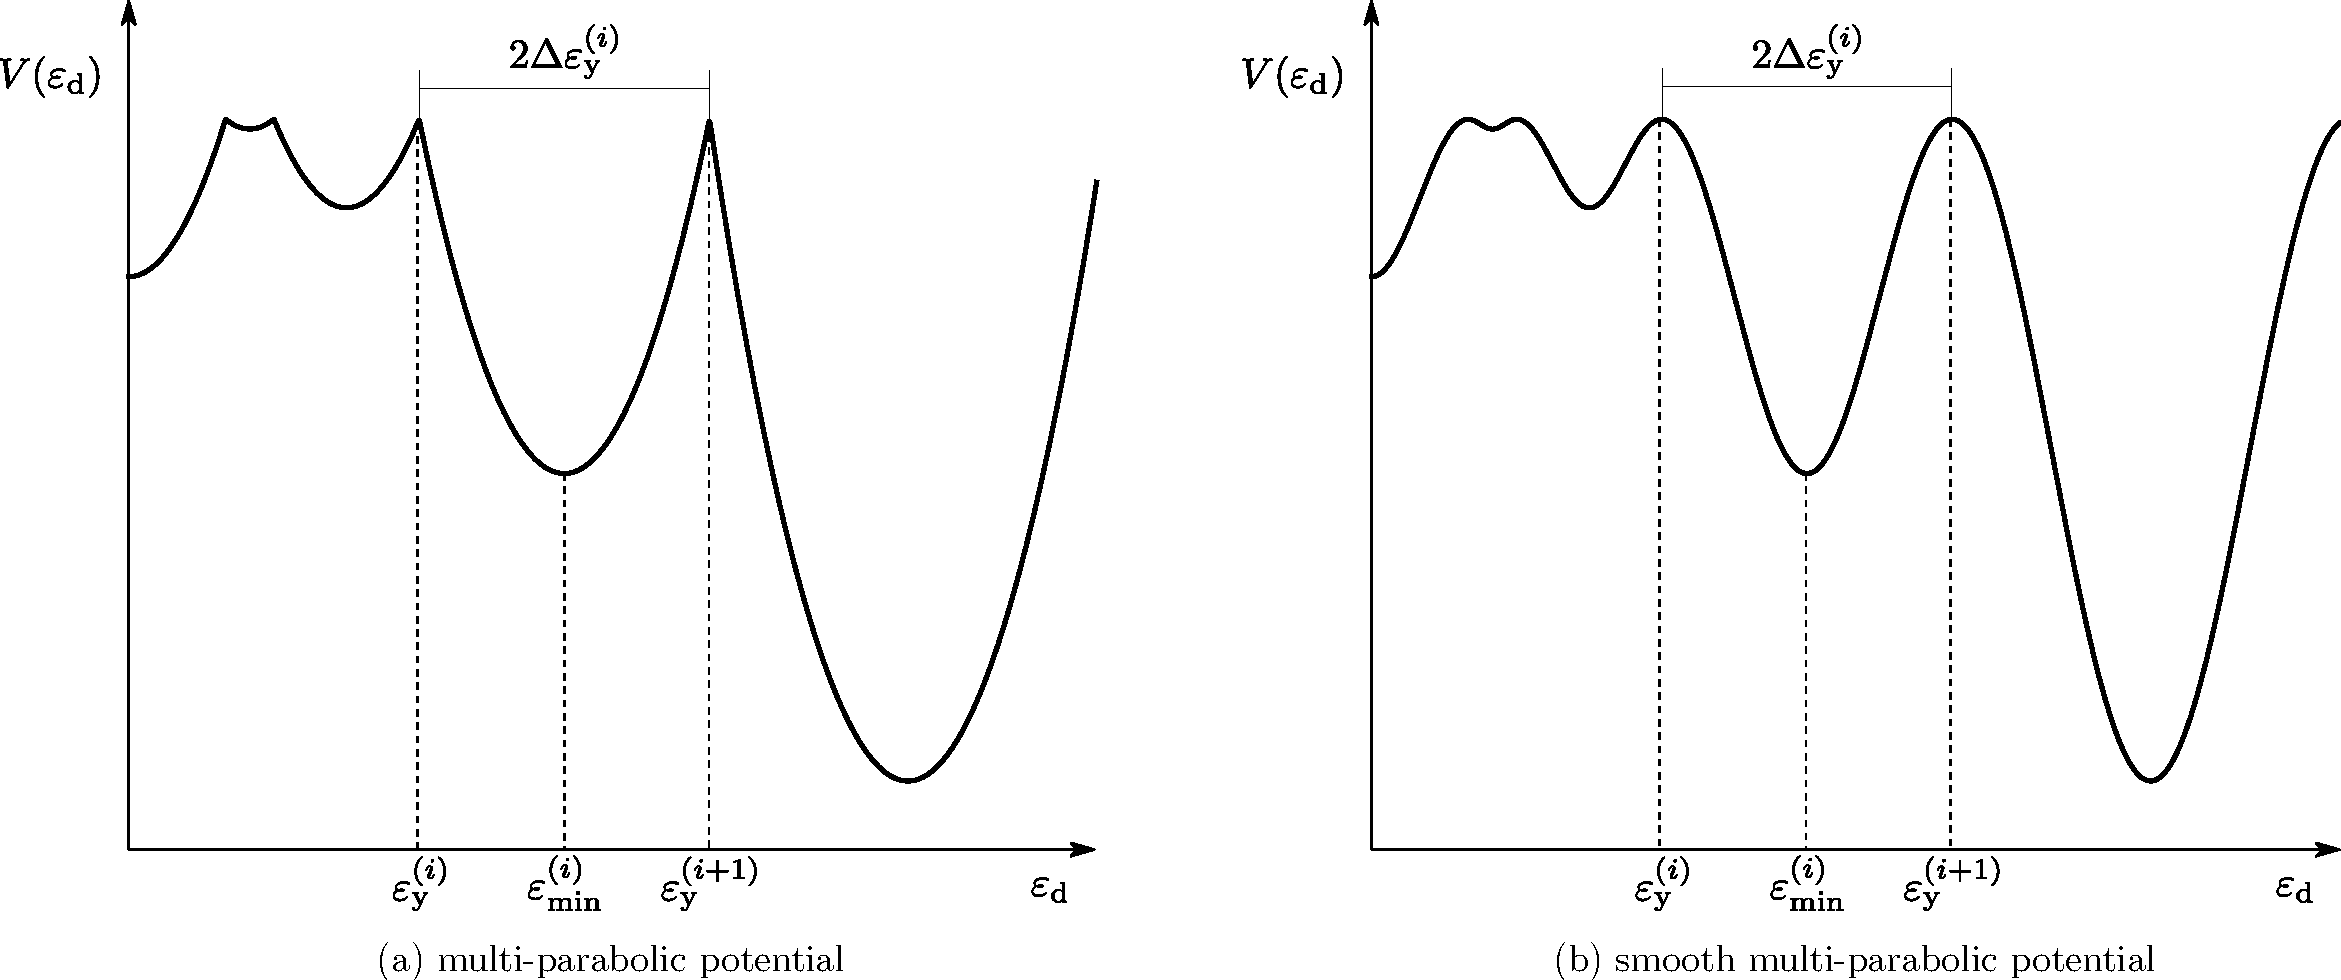
\includegraphics[width=1.\textwidth]{figures/potential_V-plas}
  \caption{The multi-minima shear strain energy, $V ( \varepsilon_\mathrm{d} )$, that models the effect of plasticity. The multi-parabolic shear strain energy is shown in (a), while its smoothened equivalent is shown in (b).}
  \label{fig:V:plas}
\end{figure}

\begin{figure}[htp]
  \centering
  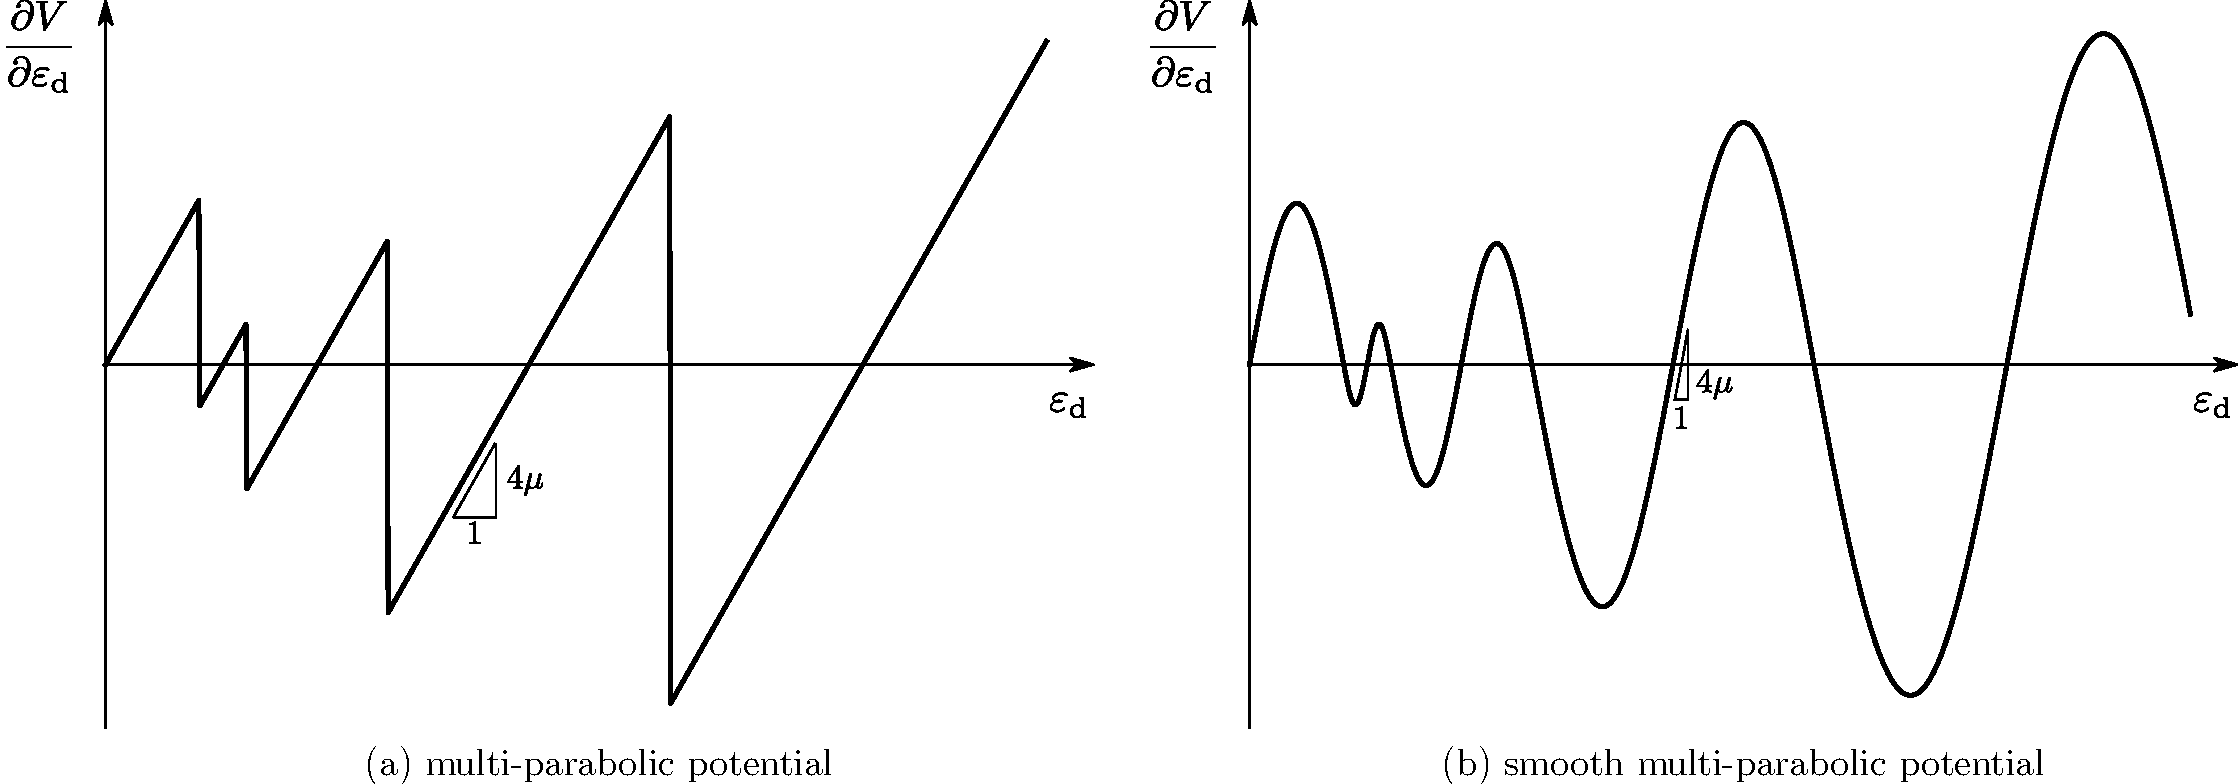
\includegraphics[width=1.\textwidth]{figures/potential_dV-plas}
  \caption{Derivative of the shear strain energy $V$.}
  \label{fig:dV:plas}
\end{figure}

\appendix

\vfill\newpage
\section{Tensors and tensor products}
\label{sec:nomenclature:tensor}

\begin{itemize}
%
\item Second order tensor
\begin{equation}
  \T{A} = A_{ij} \vec{e}_i \vec{e}_j
\end{equation}
%
\item Dyadic tensor product
\begin{align}
  \T{C} &= \vec{a} \otimes \vec{b} \\
  C_{ij} &= a_{i} \, b_{j}
\end{align}
%
\item Double tensor contraction
\begin{align}
  C &= \T{A} : \T{B} = \mathrm{tr} \left( \T{A} \cdot \T{B} \right) \\
    &= A_{ij} \, B_{ji}
\end{align}
%
\end{itemize}

\section{Unit tensors}
\label{sec:nomenclature:unit}

\begin{itemize}
%
\item Second order unit tensor
\begin{equation}
  \T{I} = \delta_{ij} \vec{e}_i \vec{e}_j
\end{equation}
It is easy to show that it has the property that
\begin{equation}
  \T{I} : \T{A} = \mathrm{tr} ( \bm{A} )
\end{equation}
%
\item Fourth order unit tensor:
\begin{equation}
  \TT{I} : \T{A} \equiv \T{A}
\end{equation}
i.e.
\begin{equation}
  \delta_{il} \delta_{jk} A_{lk} = A_{ij}
\end{equation}
hence
\begin{equation}
  \TT{I} = \delta_{il} \delta_{jk} \vec{e}_i \vec{e}_j \vec{e}_k \vec{e}_l
\end{equation}
%
\item Deviatoric projection
\begin{equation}
  \TT{I}_\mathrm{d} : \T{A} \equiv \T{A} - \tfrac{1}{3} \mathrm{tr} ( \bm{A} ) \T{I}
\end{equation}
hence
\begin{equation}
  \TT{I}_\mathrm{d} = \TT{I} - \tfrac{1}{3} \T{I} \otimes \T{I}
  = \left( \delta_{il} \delta_{jk} - \tfrac{1}{3} \delta_{ij} \delta_{kl} \right) \vec{e}_i \vec{e}_j \vec{e}_k \vec{e}_l
\end{equation}
%
\end{itemize}

\section{Strain measures}
\label{sec:nomenclature::strain}

\begin{itemize}
%
\item Volumetric strain
\begin{equation}
  \varepsilon_\mathrm{m} = \tfrac{1}{3} \mathrm{tr} ( \T{\varepsilon} )
\end{equation}
%
\item Strain deviator
\begin{equation}
  \T{\varepsilon}_\mathrm{d}
  = \T{\varepsilon} - \tfrac{1}{3} \mathrm{tr} ( \T{\varepsilon} ) \, \T{I}
  = \T{\varepsilon} - \varepsilon_\mathrm{m} \, \T{I}
  = \TT{I}_\mathrm{d} : \T{\varepsilon}
\end{equation}
%
\item Equivalent deviatoric strain
\begin{equation}
  \varepsilon_\mathrm{d}
  = \sqrt{ \tfrac{1}{2} \T{\varepsilon}_\mathrm{d} : \T{\varepsilon}_\mathrm{d} }
\end{equation}
%
\end{itemize}

\section{Stress measures}
\label{sec:nomenclature::stress}

\begin{itemize}
%
\item Hydrostatic stress
\begin{equation}
  \sigma_\mathrm{m} = \tfrac{1}{3} \mathrm{tr} ( \T{\sigma} )
\end{equation}
%
\item Stress deviator
%
\begin{equation}
  \T{\sigma}_\mathrm{d}
  = \T{\sigma} - \tfrac{1}{3} \mathrm{tr} ( \T{\sigma} ) \, \T{I}
  = \T{\sigma} - \sigma_\mathrm{m} \, \T{I}
  = \TT{I}_\mathrm{d} : \T{\sigma}
\end{equation}
%
\item Equivalent deviatoric stress
\begin{equation}
\sigma_\mathrm{d} = \sqrt{2 \T{\sigma}_\mathrm{d} : \T{\sigma}_\mathrm{d} }
\end{equation}
Note that this definition is such that the equivalent deviatoric stress and strain are work conjugate, i.e.
\begin{equation}
  \T{\sigma}_\mathrm{d} : \T{\varepsilon}_\mathrm{d} = \sigma_\mathrm{d} \varepsilon_\mathrm{d}
\end{equation}
%
\end{itemize}

\section{Derivatives}
\label{sec:nomenclature:derivatives}

\begin{itemize}
%
\item Trace of the strain
\begin{equation}
  \frac{ \partial \, \mathrm{tr} ( \T{\varepsilon} ) }{ \partial \T{\varepsilon} }
  =
  \frac{ \partial }{ \partial \T{\varepsilon} } \left( \T{\varepsilon} : \T{I} \right)
  =
  \frac{ \partial \T{\varepsilon} }{ \partial \T{\varepsilon} } : \T{I}
  =
  \TT{I} : \T{I}
  =
  \T{I}
\end{equation}
%
\item Strain deviator
\begin{equation}
  \frac{\partial \T{\varepsilon}_\mathrm{d}}{\partial \T{\varepsilon}}
  =
  \frac{ \partial }{ \partial \T{\varepsilon} } \left( \T{\varepsilon} - \tfrac{1}{3} \mathrm{tr} ( \T{\varepsilon} ) \T{I} \right)
  =
  \TT{I} - \tfrac{1}{3} \T{I} \otimes \T{I}
  =
  \TT{I}_\mathrm{d}
\end{equation}
%
\item Equivalent shear strain
\begin{equation}
  \frac{ \partial \varepsilon_\mathrm{d} }{ \partial \T{\varepsilon} }
  =
  \frac{\partial}{\partial \T{\varepsilon}} \sqrt{\tfrac{1}{2} \T{\varepsilon}_\mathrm{d} : \T{\varepsilon}_\mathrm{d}}
  =
  \frac{1}{2 \varepsilon_\mathrm{d}}
  \frac{2}{2}
  \left[\, \frac{\partial \T{\varepsilon}_\mathrm{d}}{\partial \T{\varepsilon}} : \T{\varepsilon}_\mathrm{d} + \T{\varepsilon}_\mathrm{d} : \frac{\partial \T{\varepsilon}_\mathrm{d}}{\partial \T{\varepsilon}} \,\right]
  =
  \frac{1}{4 \varepsilon_\mathrm{d}}
  \big[\, \TT{I}_\mathrm{d} : \T{\varepsilon}_\mathrm{d} + \T{\varepsilon}_\mathrm{d} : \TT{I}_\mathrm{d} \,\big]
  =
  \frac{1}{2}
  \frac{\T{\varepsilon}_\mathrm{d}}{\varepsilon_\mathrm{d}}
  \equiv
  \tfrac{1}{2}
  \T{N}_d
\end{equation}
%
\end{itemize}

\bibliography{library}

\end{document}
